%% ----------------------------------------------- %%
%%            Graphical user interface             %%
%% (documentation chapter for the FilmTit project) %%
%% ----------------------------------------------- %%

\section{Goals}
% (Honza)
Our main goal is to offer a tool for the translators of the movie subtitles as easy and effective to use as possible. With the capabilities of the current web browsers, we decided to make FilmTit a web-based application, therefore sparing the user the need to download and install anything.

\section{Google Web Toolkit}
% (Honza and Ruda)
The web-based user interface representing the client part of the FilmTit application is based on the Google Web Toolkit (GWT) framework. This technology is a development toolkit for building and optimizing browser-based applications %\citep{Gwtweb}
and is based on the idea of translation of Java source code into Javascript. Therefore, it enables us to write in Java even on the client side, but preserving most of the advantages of web application accessibility for the user.

The official description of GWT isas follows:

Google Web Toolkit (GWT) is a development toolkit for building and optimizing complex browser-based applications. Its goal is to enable productive development of high-performance web applications without the developer having to be an expert in browser quirks, XMLHttpRequest, and JavaScript. GWT is used by many products at Google, including Google Wave and the new version of AdWords. It's open source, completely free, and used by thousands of developers around the world.


\todo{probably move to Implementation Process}
We decided to use GWT for several reasons.

One reason is that it integrates very well with the rest of the application, which is written in Java. A prominent example is the communication between GUI and Userspace. Not only is the interface defined by one simple Java class (FilmTitService.java), which is then used both by the GUI and the Userspace, but thanks to GWT we are even able to use exactly the same classes (placed in share) in GUI and in Userspace and send them easily through the FilmTitService interface. Thus, we avoided the trouble of having to keep each of these classes in two versions, Java and Javascript, together with mappings to and from the transport format. In fact, all of these do exist in the application, but only in the compiled code, completely hidden from the developer.

However, there is a downside which can be expected but is difficult to manage properly. It is obvious that GWT does not support everything that exists in Java -- instead, it supports only a subset of Java, with a lot of GWT-specific additions. This is perfectly reasonable, and, as the subset supported is large enough, should not cause any problems. However, the cut between supported and unsupported features is very misty -- often a class is supported (e.g. LinkedList), but only some of its methods are implemented (e.g. one can use removeFirst(), but pop() is unsupported). Moreover, the IDE does not provide much support in this area, so often the only thing that a developer can rely on are internet forums. Luckily, GWT is used by many developers and most of the issues that we encountered had been already solved by others. Still, we spent a lot of debugging time on problems that were actually problems of GWT that had to be worked around, instead of being problems of our code.

A requirement that we had for the web technology was to offer an IDE (in GWT realized by a plugin for Eclipse IDE, similarly applicable also for IntelliJ IDE), possibly with debugging support. In GWT, there is a dedicated Development Mode for these debugging purposes, sparing the developer the need of recompiling all the GWT code for testing after each change. This proved to be very efficient in the first phases of the development when the GUI module was developed independently and although it turned out to be quite difficult to set up once this module was integrated with the rest of the project, it remained one of the most useful features of GWT.

Another option that we found useful is the possibility to directly insert real Javascript code into GWT methods. Although it is not very clean and cannot benefit from some of the features of GWT, it is sometimes the only way how to do something that is supported in Javascript but unsupported in GWT.

An important point also was that GWT is freeware (it is even open-source, but we did not benefit from it much), or more precisely, is licensed under the Apache License, v.~2.0 (TODO: citation for the license!), with several third-party software included in its distribution under other freeware licenses.

Although GWT can be integrated into a Maven project, it was far from flawless and a lot of time had to be spent on making everything work together, including maintaining the IDE support. We managed to do that in the end, but we had expected this to be much easier. The main reason (but not the only one) is the specific directory structure, different for the Maven project and for the GWT project, which has to be adjusted in the configuration of both the Maven plugins and the IDE.

To conclude, we are happy that we decided to use GWT because of the benefits it brought to us, but we were disappointed by the number of complications that it brought as well. Were we to decide on a web framework to use for a similar project, we would still have to consider our decision carefully.

\subsection{Browser Support and Optimization}
GWT also provides a feature which makes the final web application similar in different major browsers and optimized to a certain degree for each of them. This feature is called {\em deferred binding} and it is based on generating different versions of the Javascript code during compile time, only one of which needs to be loaded by a particular client browser at runtime. This process is by default maintained by the GWT compiler itself, so that the developer does not have to worry about it.

However, this ``unification'' is not complete, nor it is intended to be. It covers only the bigger and more crucial differences of the code behaviour among various browsers, but does not address some slight variancies e.g. in design of the basic elements (and their most common behaviour). This seems reasonable, because forcing each browser to interpret the code in the exact same way would mean hardcoding almost everything from scratch and not using many of their provided features, which would be probably impossible anyway. Nevertheless, some of these ``slight differences'' which we have encountered proved to be quite crucial for our intended design (especially in the event-handling domain), so lots of work had to be done to reasonably unify the application's behaviour even among the major browsers.

Still, our hope is that GWT development will continue and will keep up with the development of web browsers, allowing us to provide browser-up-to-date versions of FilmTit simply by acquiring a new version of GWT and recompiling the project.

TODO: FilmTit actual browser support -- tested and optimized for what? (here or somewhere else?)

\subsection{Designing by UiBinder}
Another very useful and comfortable feature of the GWT for designing the user interface is the UiBinder. The idea behind this approach is to design the visual structure of the page (or its part) in an HTML-like way (this is called the {\em UiBinder template}) and its behaviour and functionality in a Java class (called the {\em owner class} for the template). The UiBinder itself is then an object binding these two approaches together. This style of creating the web application supports the respected best practice to divide the visual design and the functionality. It also allows to create the web page's appearance in a way which is more natural to web designers (e.g. HTML-like), as well as more readable and modifiable. Other advantages includes supposedly better performance (as the browsers can better optimize the rendering from the UiBinder templates than from the heavier-weight Java-based widgets and panels) and support for internationalization (not used by FilmTit at the moment).

The actual source code of a page designed this way (or of its segment) then consists of a file with the *.ui.xml Ui-Binder template (where also the style definition can be included directly) and a corresponding *.java owner class, where the elements of the template can be accessed as widgets (as well as made accessible to other classes). The owner class then can be simply instantiated and plugged into an existing design just like any other widget.

\subsection{Twitter Bootstrap Library}
For enhancing the visual appearance of our application to a modern look without a professional graphic designer, we have decided to use an existing open-source library for GWT which displays the page elements (and their groups) in the style of the Twitter pages. This library is called GWT-Bootstrap and is easily applicable with the UiBinder-style designing. It is also still a live project, so there is a hope that more features would be available in the possible future development.

Similarly to other third-party libraries used by FilmTit, the GWT-Bootstrap library is attached as a Maven dependency and downloaded automatically from its own Maven repository.


\section{GUI Structure}
% (Honza/Ruda)

package cz.filmtit.client (not cz.filmtit.gui for historical reasons -- ``client'' is the default package name in GWT for the client side of a web application)

Some settings have to be done via several resource files in the webapp directory. (This is required by the Java Servlets technology used to deploy the application.)

\todo{I already wrote a lot into the implementation process and I dont want to have duplicities in the documentation, so I am now keeping the development description in implementation process but moving detailed descriptions of the final solution from implemenattion process into this section. Prosim bud pacient :-)}

\subsection{Gui.java}

The main class is Gui.java. It defines the web application itself, providing an entry point, initialization methods and logging methods. It also handles general requests.

\subsection{Pages}

subpackage cz.filmtit.client.pages

Please refer to the sitemap figure \ref{fig:sitemap} for an overview of all pages.

\begin{figure}
\begin{center}
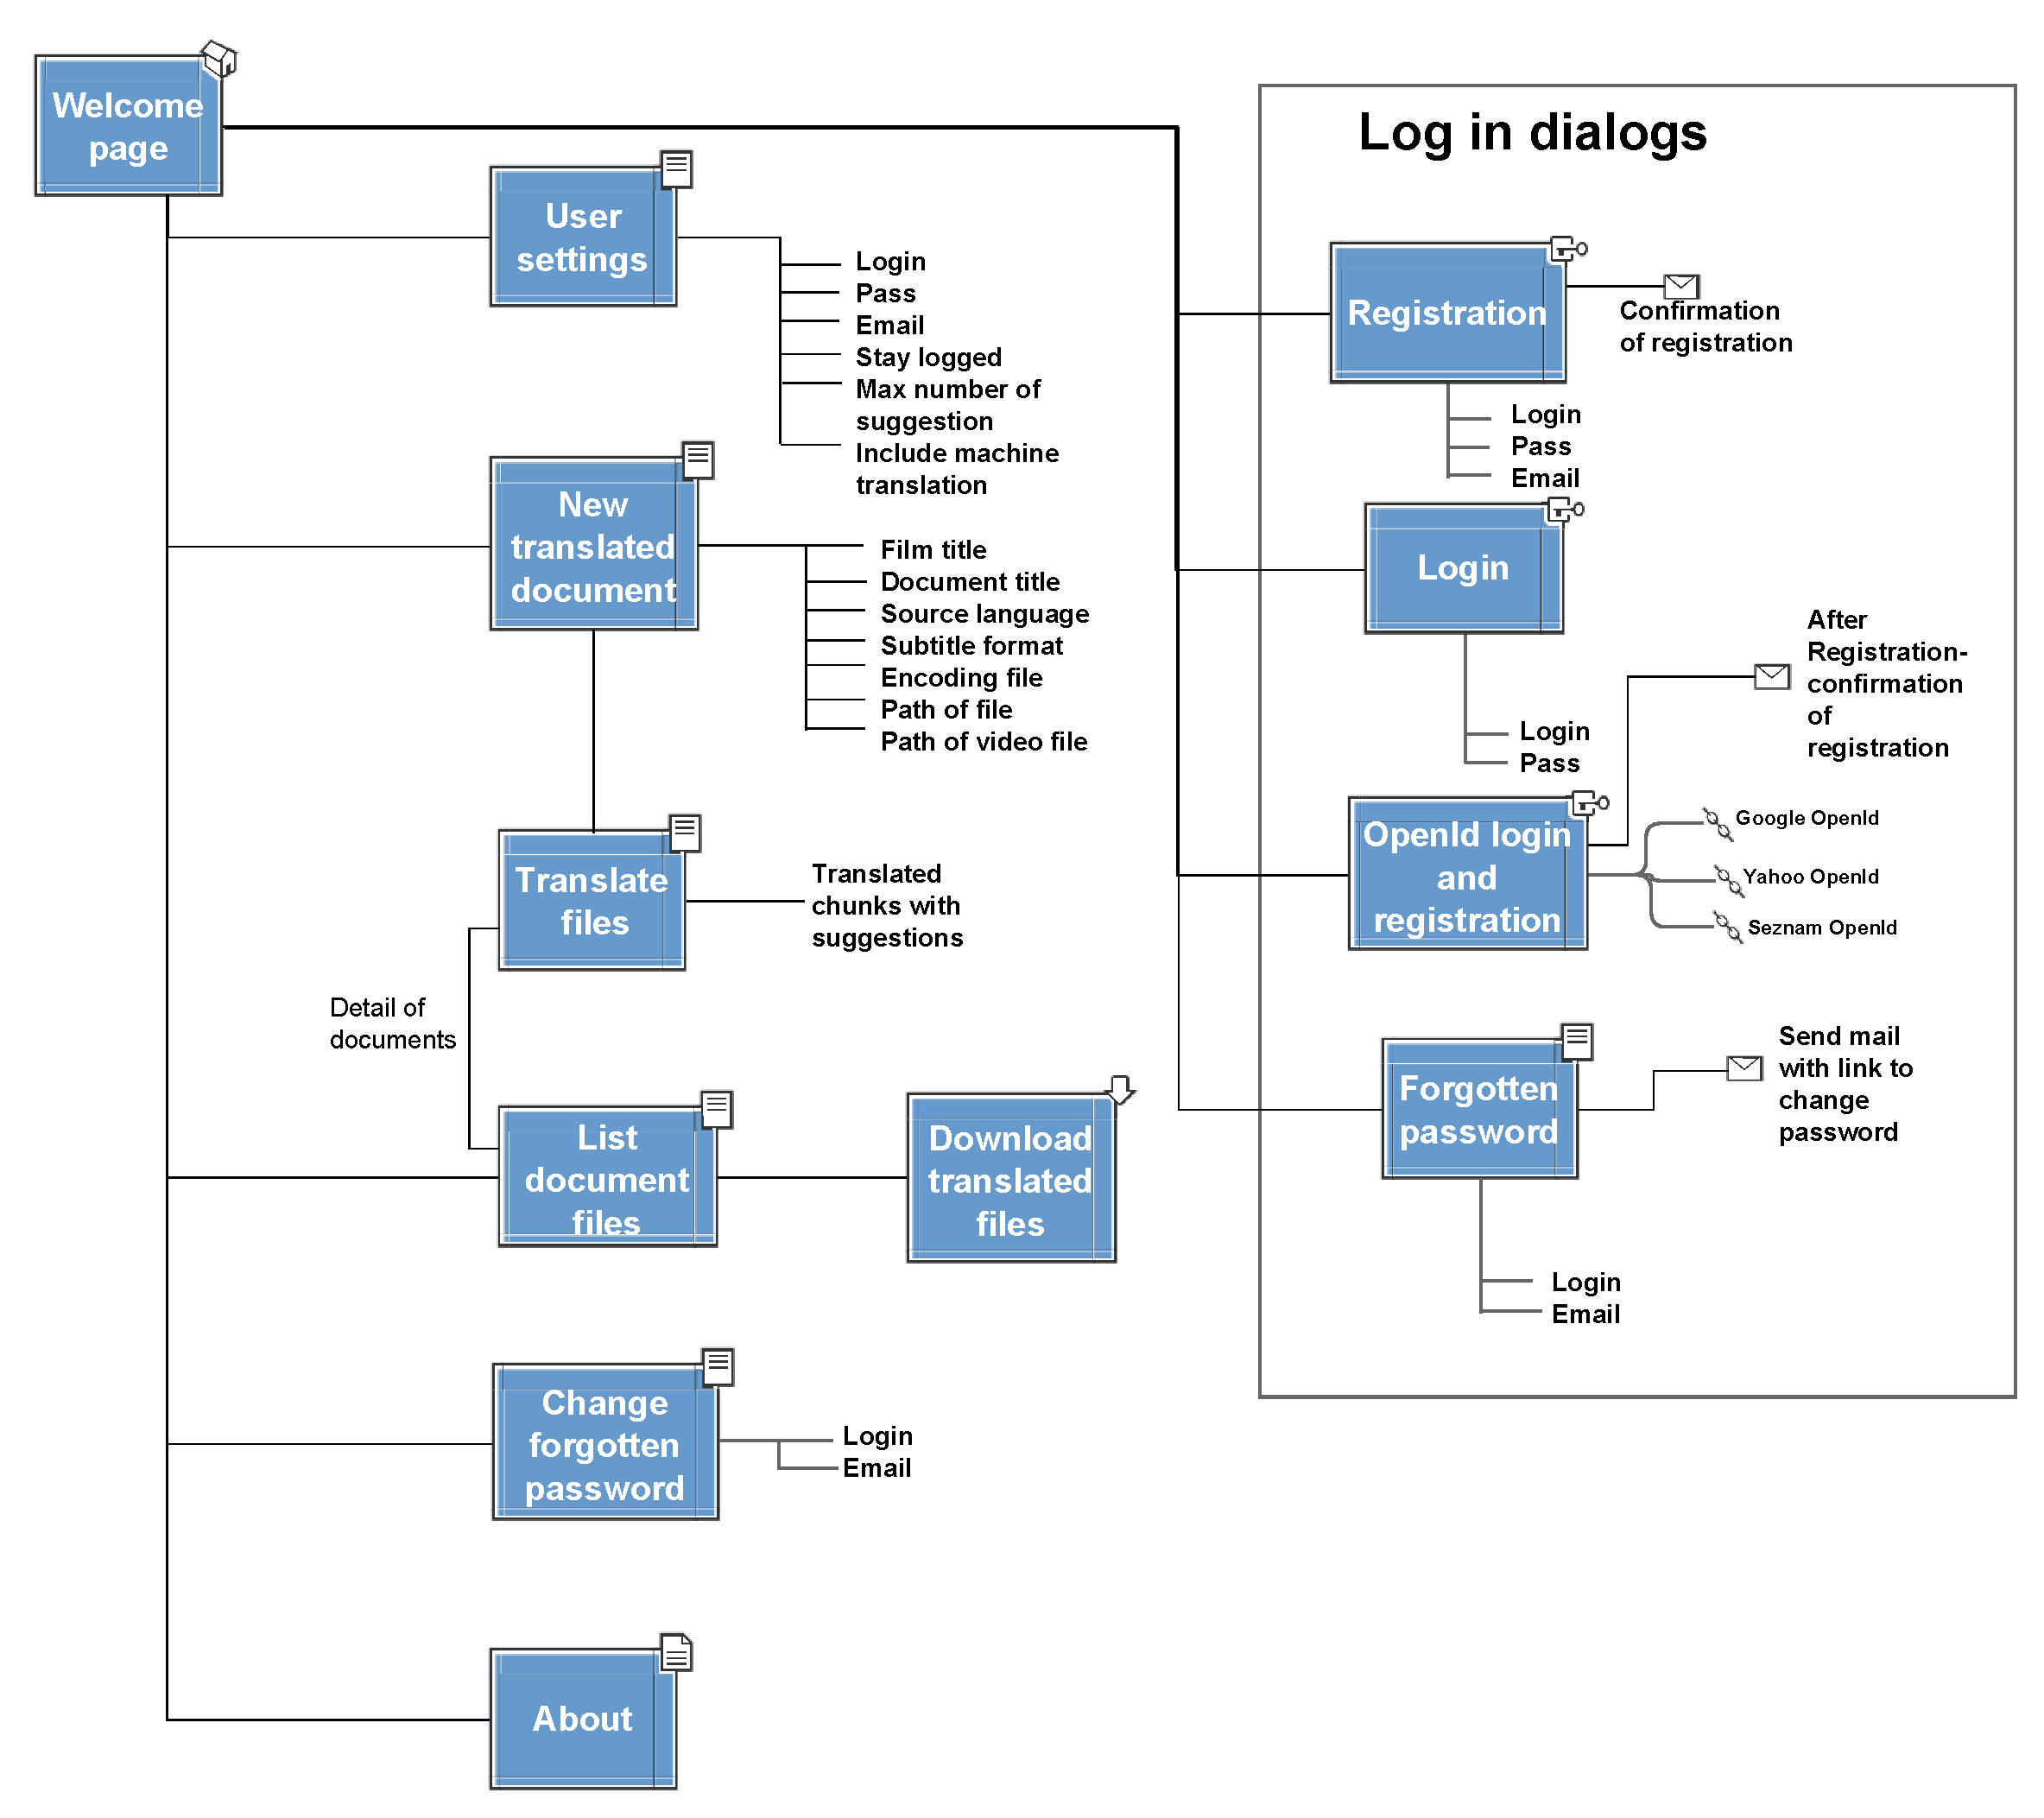
\includegraphics[scale=0.4]{figures/sitemap.pdf}
\end{center}
\caption{Site map of the application}
\label{fig:sitemap}
\end{figure}

layout defined by UiBinder

page is created and loaded by calling its constructor, which may require some parameters (such as documentID for TranslationWorkspace)

page loading and switching handled by PageHandler; also provides support for URLs: e.g. the About page can be accessed by a URL http://server/\#About or http://server/?page=About (the first one being the default), with the help of the History class

GuiStructure -- defines menu and the content panel, handles menu activation/deactivation, shows the login/logout link

\subsubsection{TranslationWorkspace}

maybe describe in more detail, maybe not

\subsection{Dialogs}

subpackage cz.filmtit.client.dialogs

typically extended from Dialog

defines deactivate(), reactivate(), showInfoMessage() and showErrorMessage(); all dialogs should only be accessed via this interface (except for their creatin, which is invoked by their constructor)

typically use a Modal 

\subsection{Remote Procedure Calls Implementation}

subpackage cz.filmtit.client.callables

Each call represented by an instance of a class with the name similar to the RPC name (e.g. for deleteDocument RPC it is the DeleteDocument class), extended from Callable.

Callable:

-- to alleviate the burden of boiler-plate code

-- to provide utility methods and default actions (logging, error handling)

The superclass also provides logging for all the requests, based on the classname and the parameters of the subclass.

-- to provide a common structure for all RPCs

E.g. RPC deleteDocument(sessionID, documentID)
is invoked as new DeleteDocument(sessionID, documentID).

the callback is defined by the class

wrappers for the ``raw'' RPC calls

The subclasses representing the individual calls must only override the call() method, which specifies the actual RPC to be invoked.
They can also modify the default behavior defined by the superclass by overriding several other methods, such as onSuccessAfterLog, onEachReturn, onFailureAfterLog, onProbablyOffline etc. This way, the behavior needed can be always achieved, but the default implementation is often sufficient, so the subclasses often override only one or two methods, keeping their code as simple as possible. (The method most often overridden is the onSuccessAfterLog method; its default implementation is to do nothing, which is only good for RPCs that do not require any reaction of GUI on their successful return, such as changeDocumentTitle or stopTranslationResults.)

\subsubsection{Error Handling}

If the request fails for any reason, it is retried by default; four attempts are made for each request, always retrying after a short time interval.
Resending the request is the default behavior which the subclasses override in cases where it is obvious that resending will not help (e.g. incorrect e-mail address format or an already existing username on registration).

In case of network problems, both temporary and permanent (this cannot be easily distinguished), the GUI usually receives a StatusCodeException with the status code 0. In such case the request is always resent three times before passing control to the onProbablyOffline method (this behavior cannot be overridden).

There is also a timeout for each request after which the request is regarded as lost and is retried.

The default action in case of an error is to show the error message in a Javascript alert window, except for the InvalidSessionIdException where the default action is to ask the user to log in again.
The subclasses often override this by showing the message in a Dialog (invoking the reactivateWithErrorMessage method of the Dialog class), or by ignoring the error completely (e.g. when deleting a document, a failure with an InvalidDocumentIdException, meaning that the document does not exist, is an error, but there is no need to inform the user because the result is the same as if the RPC succeeded: the document does not exist now.)

Most of the RPCs contain the SessionID as one of their parameters to authenticate the user. All of such RPCs can thus throw an InvalidSessionIdException, to which the default action is to show the Login Dialog to the user.

\subsection{Offline Mode}

\todo{keep everything here or describe Offline Mode in a separate section?}

Logics separated into LocalStorageHandler, Storable interface and classes implementing the interface, i.e. the SetUserTranslation class.

\subsubsection{Local Storage}

\todo{some description}

each object stored as a pair of a unique string key and a string value -- proper serialization necessary

each object defines its serialization such that its key uniquely identifies the object and the value contains all data needed to reconstruct the object which are not contained in the key

the key and value are expected to consist of semicolon separated fields by default, but each class can define its own serialization, there are no restrictions

The key is then enriched by adding the classID (e.g. ``SetUserTranslation'') and the userID (a long),
so the resulting format of key is:

full key = userID@classID:key

(the value is defined solely by the implementing class)

\subsubsection{Storable interface}

Defines methods that need to be implemented by a class to be storable in the Local Storage, especially:

\begin{itemize}
\item toKeyValuePair() -- serializes the object into a pair of a key and a value

\item static fromKeyValuePair(KeyValuePair) -- a factory method that serializes the object into a pair of a key and a value (not actually defined by the interface;  for a discussion on that matter see Implementation Process \todo{ref})

\item onLoadFromLocalStorage() -- invoked by the LocalStorageHandler when the user decides to upload the object
\end{itemize}

This interface is only implemented by the SetUserTranslation class, for reasons described in the Implementation Process \todo{ref}.

\todo{describe the serialization}

key = documentId;chunkId;partNumber

value = chosenTranslationPair;userTranslation

\subsubsection{LocalStorageHandler}

Handles storing and loading of Storable objects to and from the Local Storage.

Boolean online -- determines whether user is in Offline Mode. Setting this value is eqivalent to switching the Offline Mode on or off.

It implements especially the following methods:

\begin{itemize}
\item storeInLocalStorage (Storable) -- take a Storable object, serializes it and stores it into the Local Storage

\item loadUserObjectsFromLocalStorage() -- examine the Local Storage and return a list of objects that belong to the current user

\item uploadUserObjects() -- deserialize the loaded objects and invoke their onLoadFromLocalStorage() methods
\end{itemize}

\subsubsection{The Offline Mode operation}

\todo{here or in typical usage?}

see \ref{gui:sd:offline_mode_1} for the first phase, where the user goes offline and continues working on the translation, and \ref{gui:sd:offline_mode_2} for the second phase, where the user goes online again and the locally stored data are uploaded to the server.
(For simplicity does not show some implementation details
and, parameters are listed only if they are necessary for understanding the process.)

\begin{figure}[h]
\begin{center}
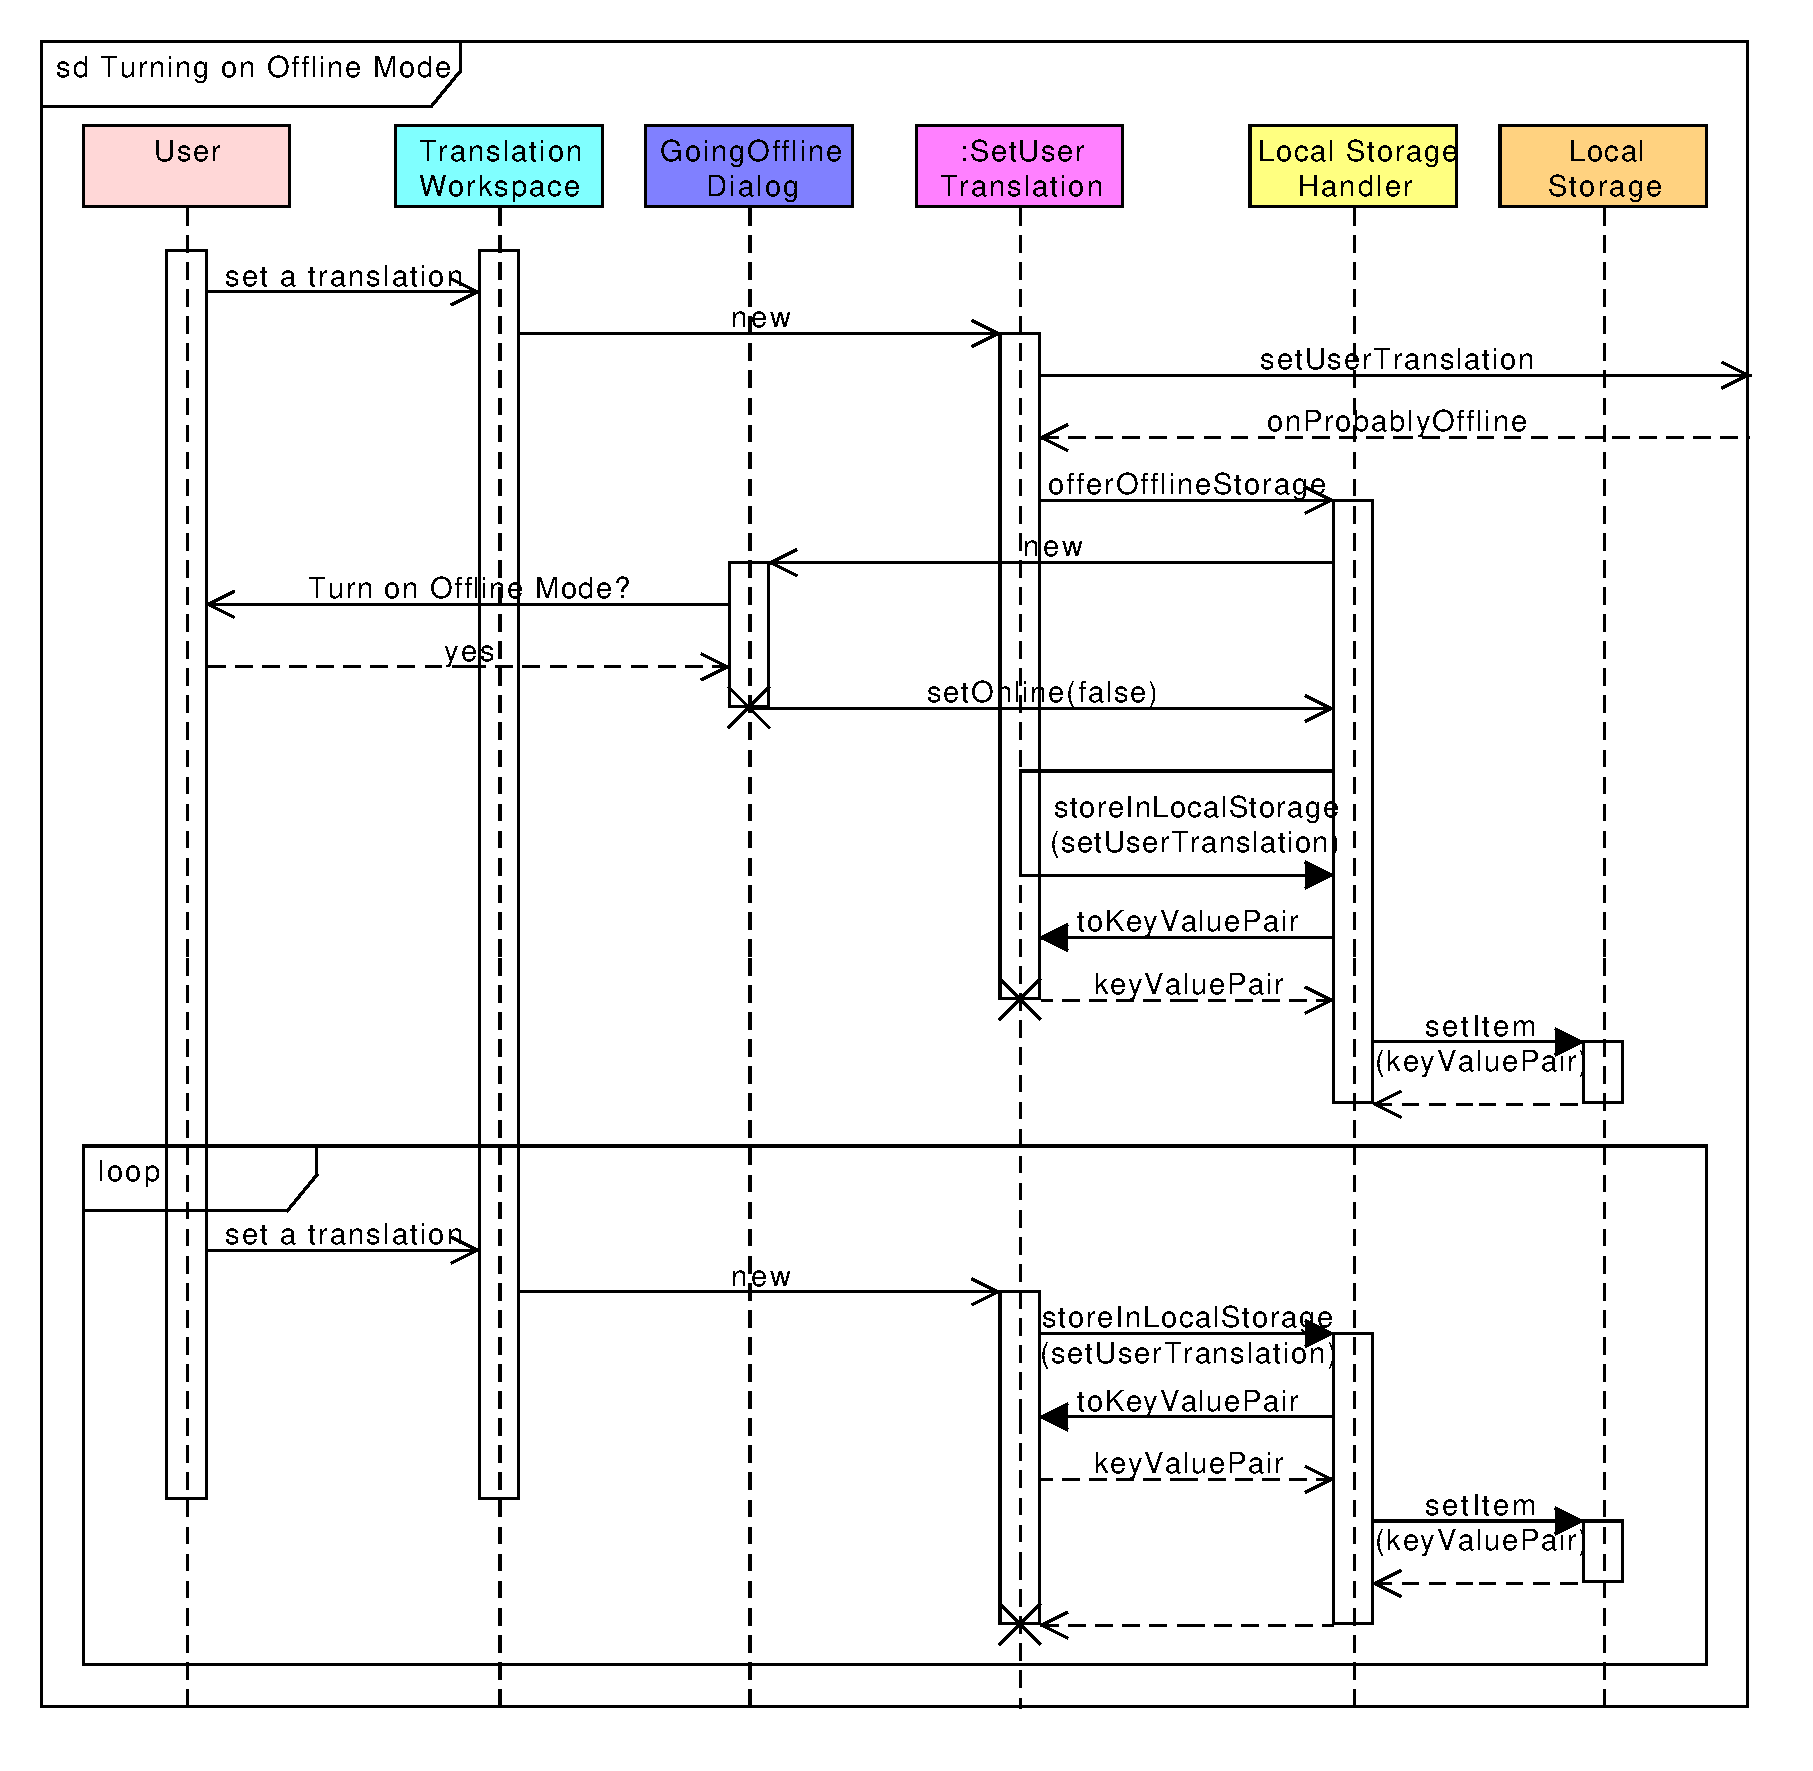
\includegraphics[scale=0.55]{figures/offline_mode_1.pdf}
\end{center}
\caption{Sequence diagram of turning on the Offline Mode and translating the document in Offline Mode.}\label{gui:sd:offline_mode_1}
\end{figure}

\begin{figure}[h]
\begin{center}
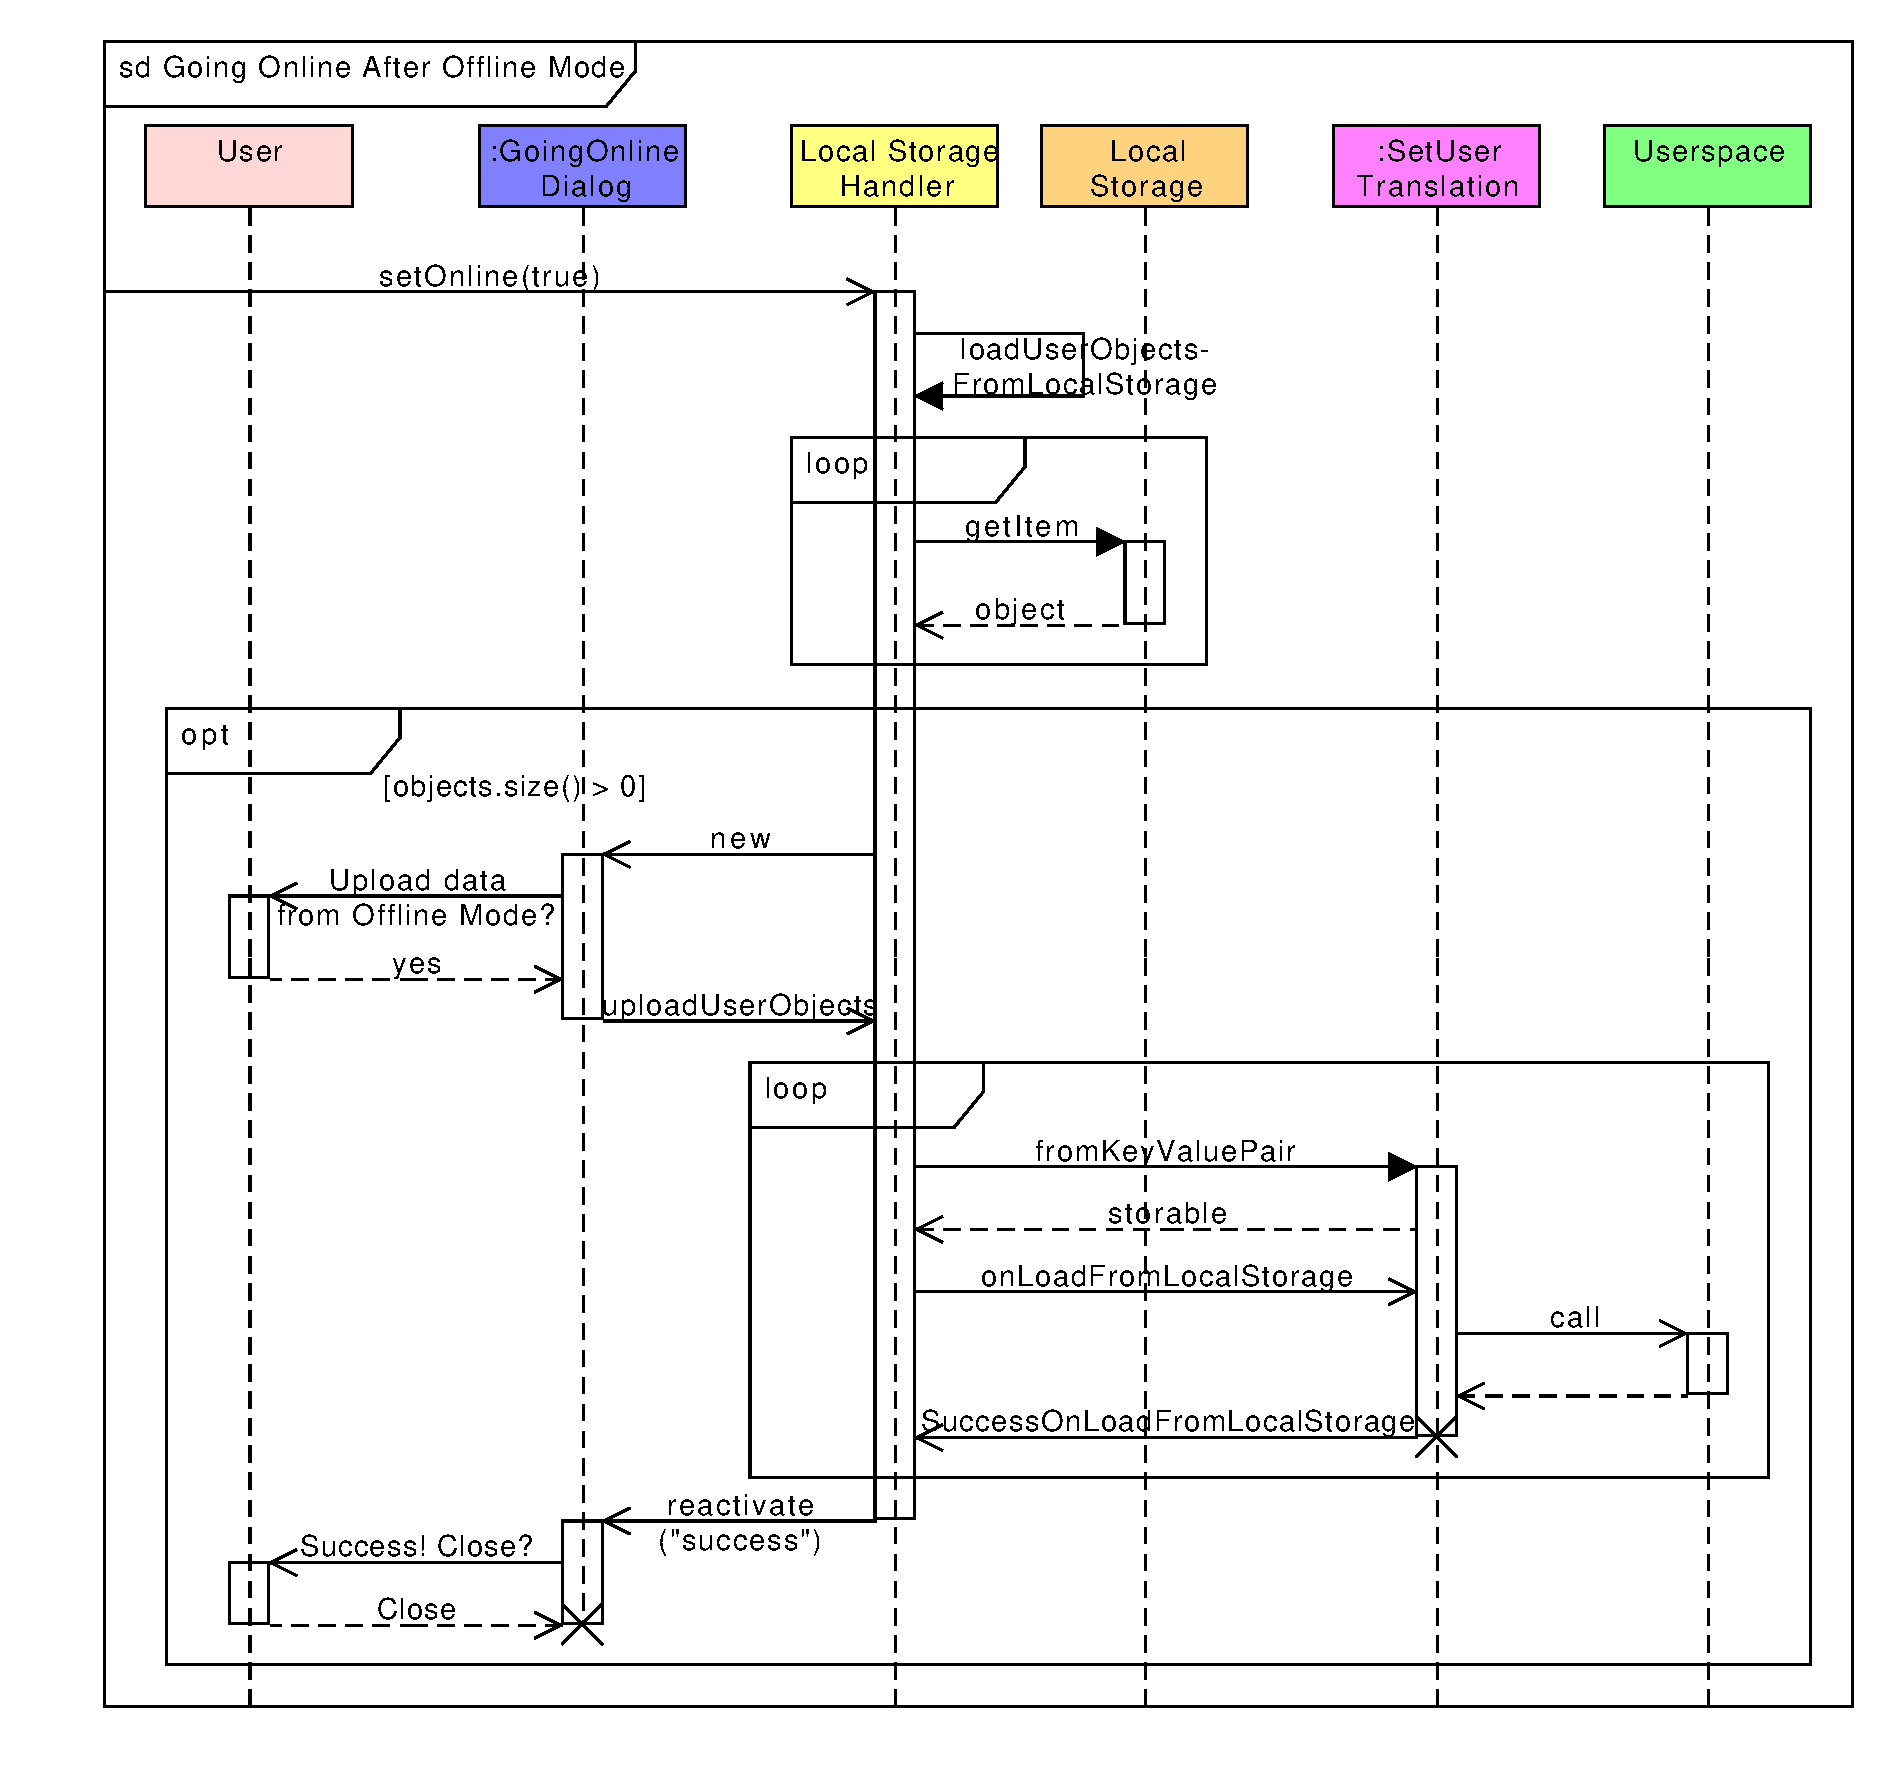
\includegraphics[scale=0.55]{figures/offline_mode_2.pdf}
\end{center}
\caption{Sequence diagram of the user going online after using Offline Mode.}\label{gui:sd:offline_mode_2}
\end{figure}

Before using the Local Storage, it is checked whether it is supported -- if it is not, Offline Mode is not offered to the user and a relevant message is displayed.

When a setUserTranslation call fails with the ``probably offline'' error, it is saved into a queue of failed calls that are to be stored offline if the user agrees (other setUserTranslation calls could already have been invoked and will also fail). If the user decides to turn on the Offline Mode, all calls from the queue are stored into Local Storage.


In Offline Mode, the style of the menu is changed and all active components are hidden, because the user should not leave the Translation Workspace while in Offline Mode. Also, going back or forward using the browser controls is disabled: each upcoming page switch is cancelled.

The SetUserTranslation calls invoked while in Offline Mode are not sent to server, but they are serialized into a key-value pair and stored in the Local Storage.


Once the user is back online and logs in again, the LocalStorageHandler examines the Local Storage. It strips the userID part of the key of each object found and compares it to the currently logged in user. If some data belonging to the user are found, he is informed about their count and is suggested to upload the data. If he agrees, LocalStorageHandler goes through the data, stripping off the ClassID and invoking the corresponding ``ClassID.fromKeyValuePair()'' deserialization. Subsequently, the onLoadFromLocalStorage() method is invoked on each of the resulting objects -- the SetUserTranslation implementation of this method is to invoke the setUserTranslation call, i.e. to store the translation on the server. When the call returns, LocalStorageHandler.SuccessOnLoadFromLocalStorage() or LocalStorageHandler.FailureOnLoadFromLocalStorage() is called, as required.

When each of the loaded objects has either succeeded or failed, the user is informed about the result. In case of errors, he can decide to retry loading the failed data or to delete them.

\subsection{SubgestBox}

subpackage cz.filmtit.client.subgestbox

An important class is the SubgestBox, or ``SUBtitle sugGESTion BOX'', which visualizes the TM results, offering a variety of means of navigation through them.

\subsection{FileLoadWidget}

subpackage cz.filmtit.client.widgets

a Widget which is a wrapper for a Java applet

\todo{Karel should proudly describe what he did}

\subsection{Video Playback (VLCWidget)}

ensured by the VLCWidget, which is a Widget wrapper to the VLC plugin

subpackage cz.filmtit.client.widgets

\todo{Karel should proudly describe what he did}

\subsection{Parsing and segmentation}
% (maybe Karel?)

\section{Typical Usage}
% (Honza)

\todo{update, some things changed...}

\subsection{Document Creation}

In the most typical case, a new user (already registered) will open the page with FilmTit and log in. Then, a dialog appears to create a new document corresponding to one movie, or more precisely, one subtitle file being translated from one language to another. Within this dialog, the user should specify which movie it is (title and year), what language pair will the translation be operating upon (e.g. from English to Czech) and provide the actual local file with the source subtitles. These information are sent to the Userspace and after refining the movie specification, the new document is created and the "translation working space" is filled with source subtitles (segmented to so-called "chunks") on the left side (as well as their timing) and corresponding empty text-boxes on the right side.

See \ref{gui:sd:document_creation}

\begin{figure}[h]
\begin{center}
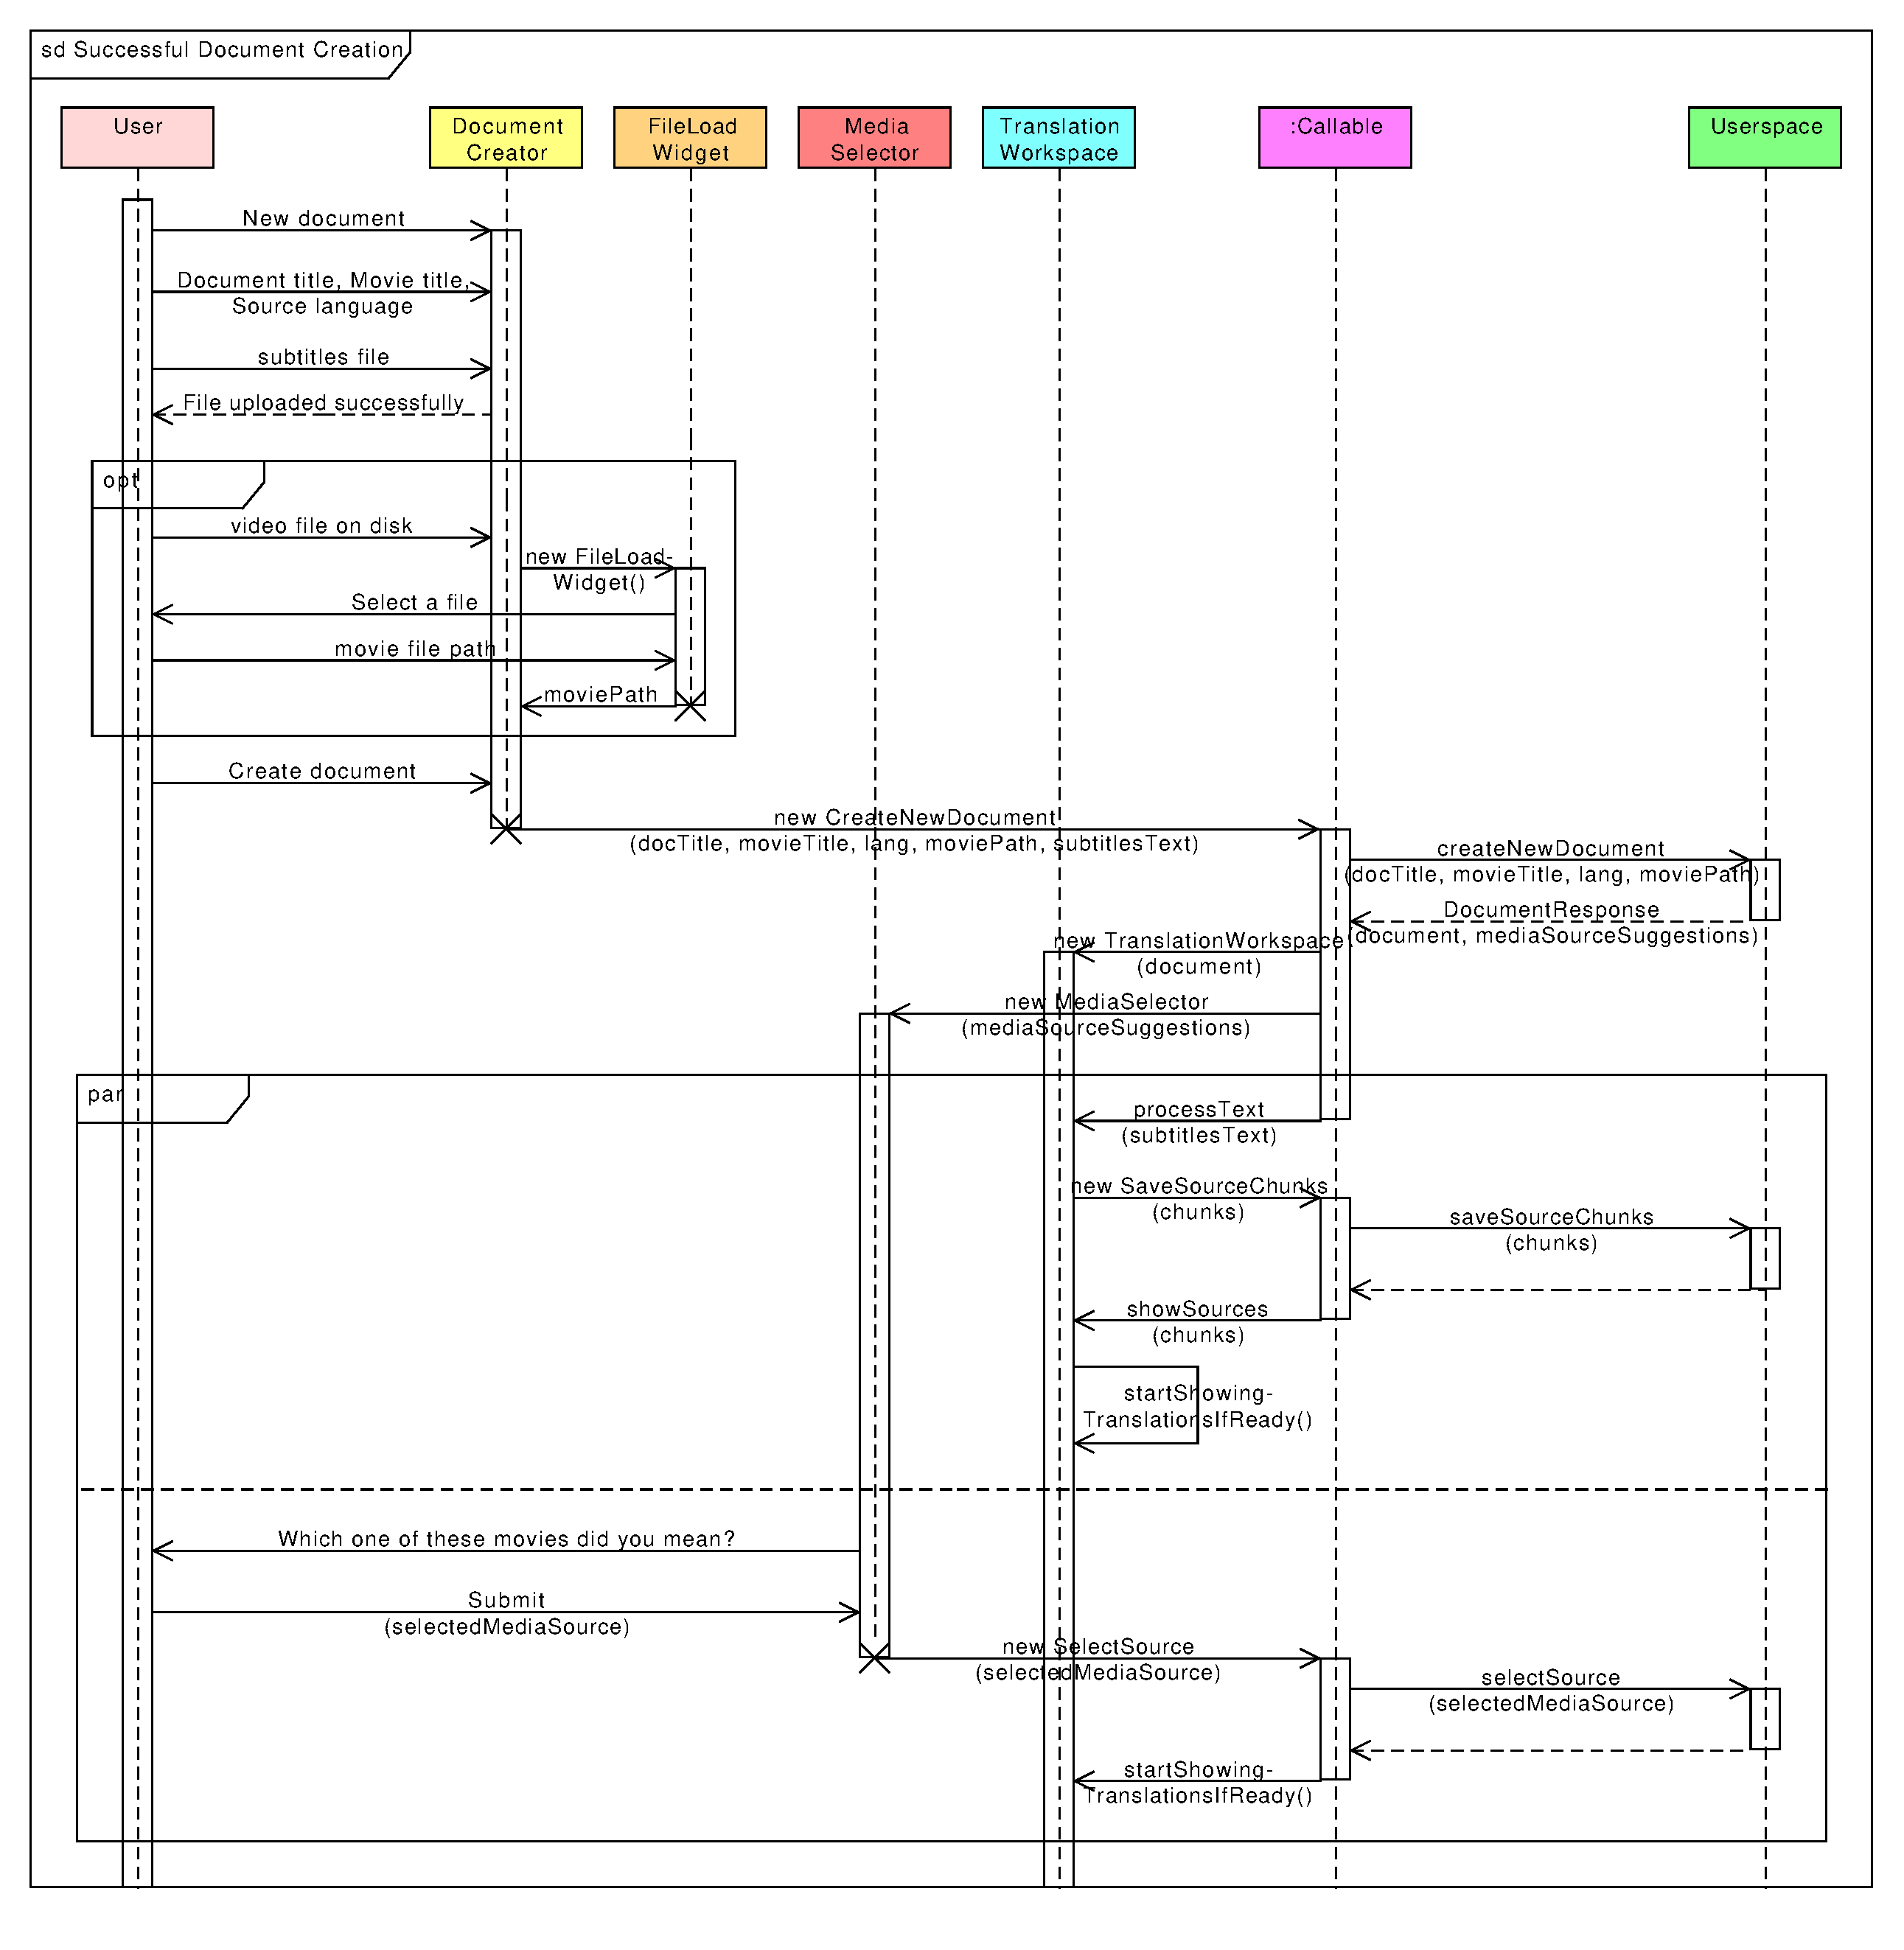
\includegraphics[scale=0.40]{figures/document_creation_sequence_GUI.pdf}
\end{center}
\caption{Sequence diagram of document creation.}\label{gui:sd:document_creation}
\end{figure}

\subsection{Document Translation}

At the same time, the subtitle chunks are sent through the Userspace to the Core, where the appropriate suggestions are generated for them and sent back. When received in the GUI, the suggestions are displayed as some kind of suggest-box, or pop-up to the corresponding text-box for the given chunk, and sorted according to their supposed accuracy (still TODO). The user can then choose any one of them (or none) and edit it (if necessary) to get the desired translation of the particular chunk. When the user leaves the chunk to the next one, his translation is sent to the Userspace to be saved here as an intermediate translation of this chunk (???also to the Core???).

See \ref{gui:sd:document_translation}
(Some technical details are ommitted for simplicity.)

\begin{figure}[h]
\begin{center}
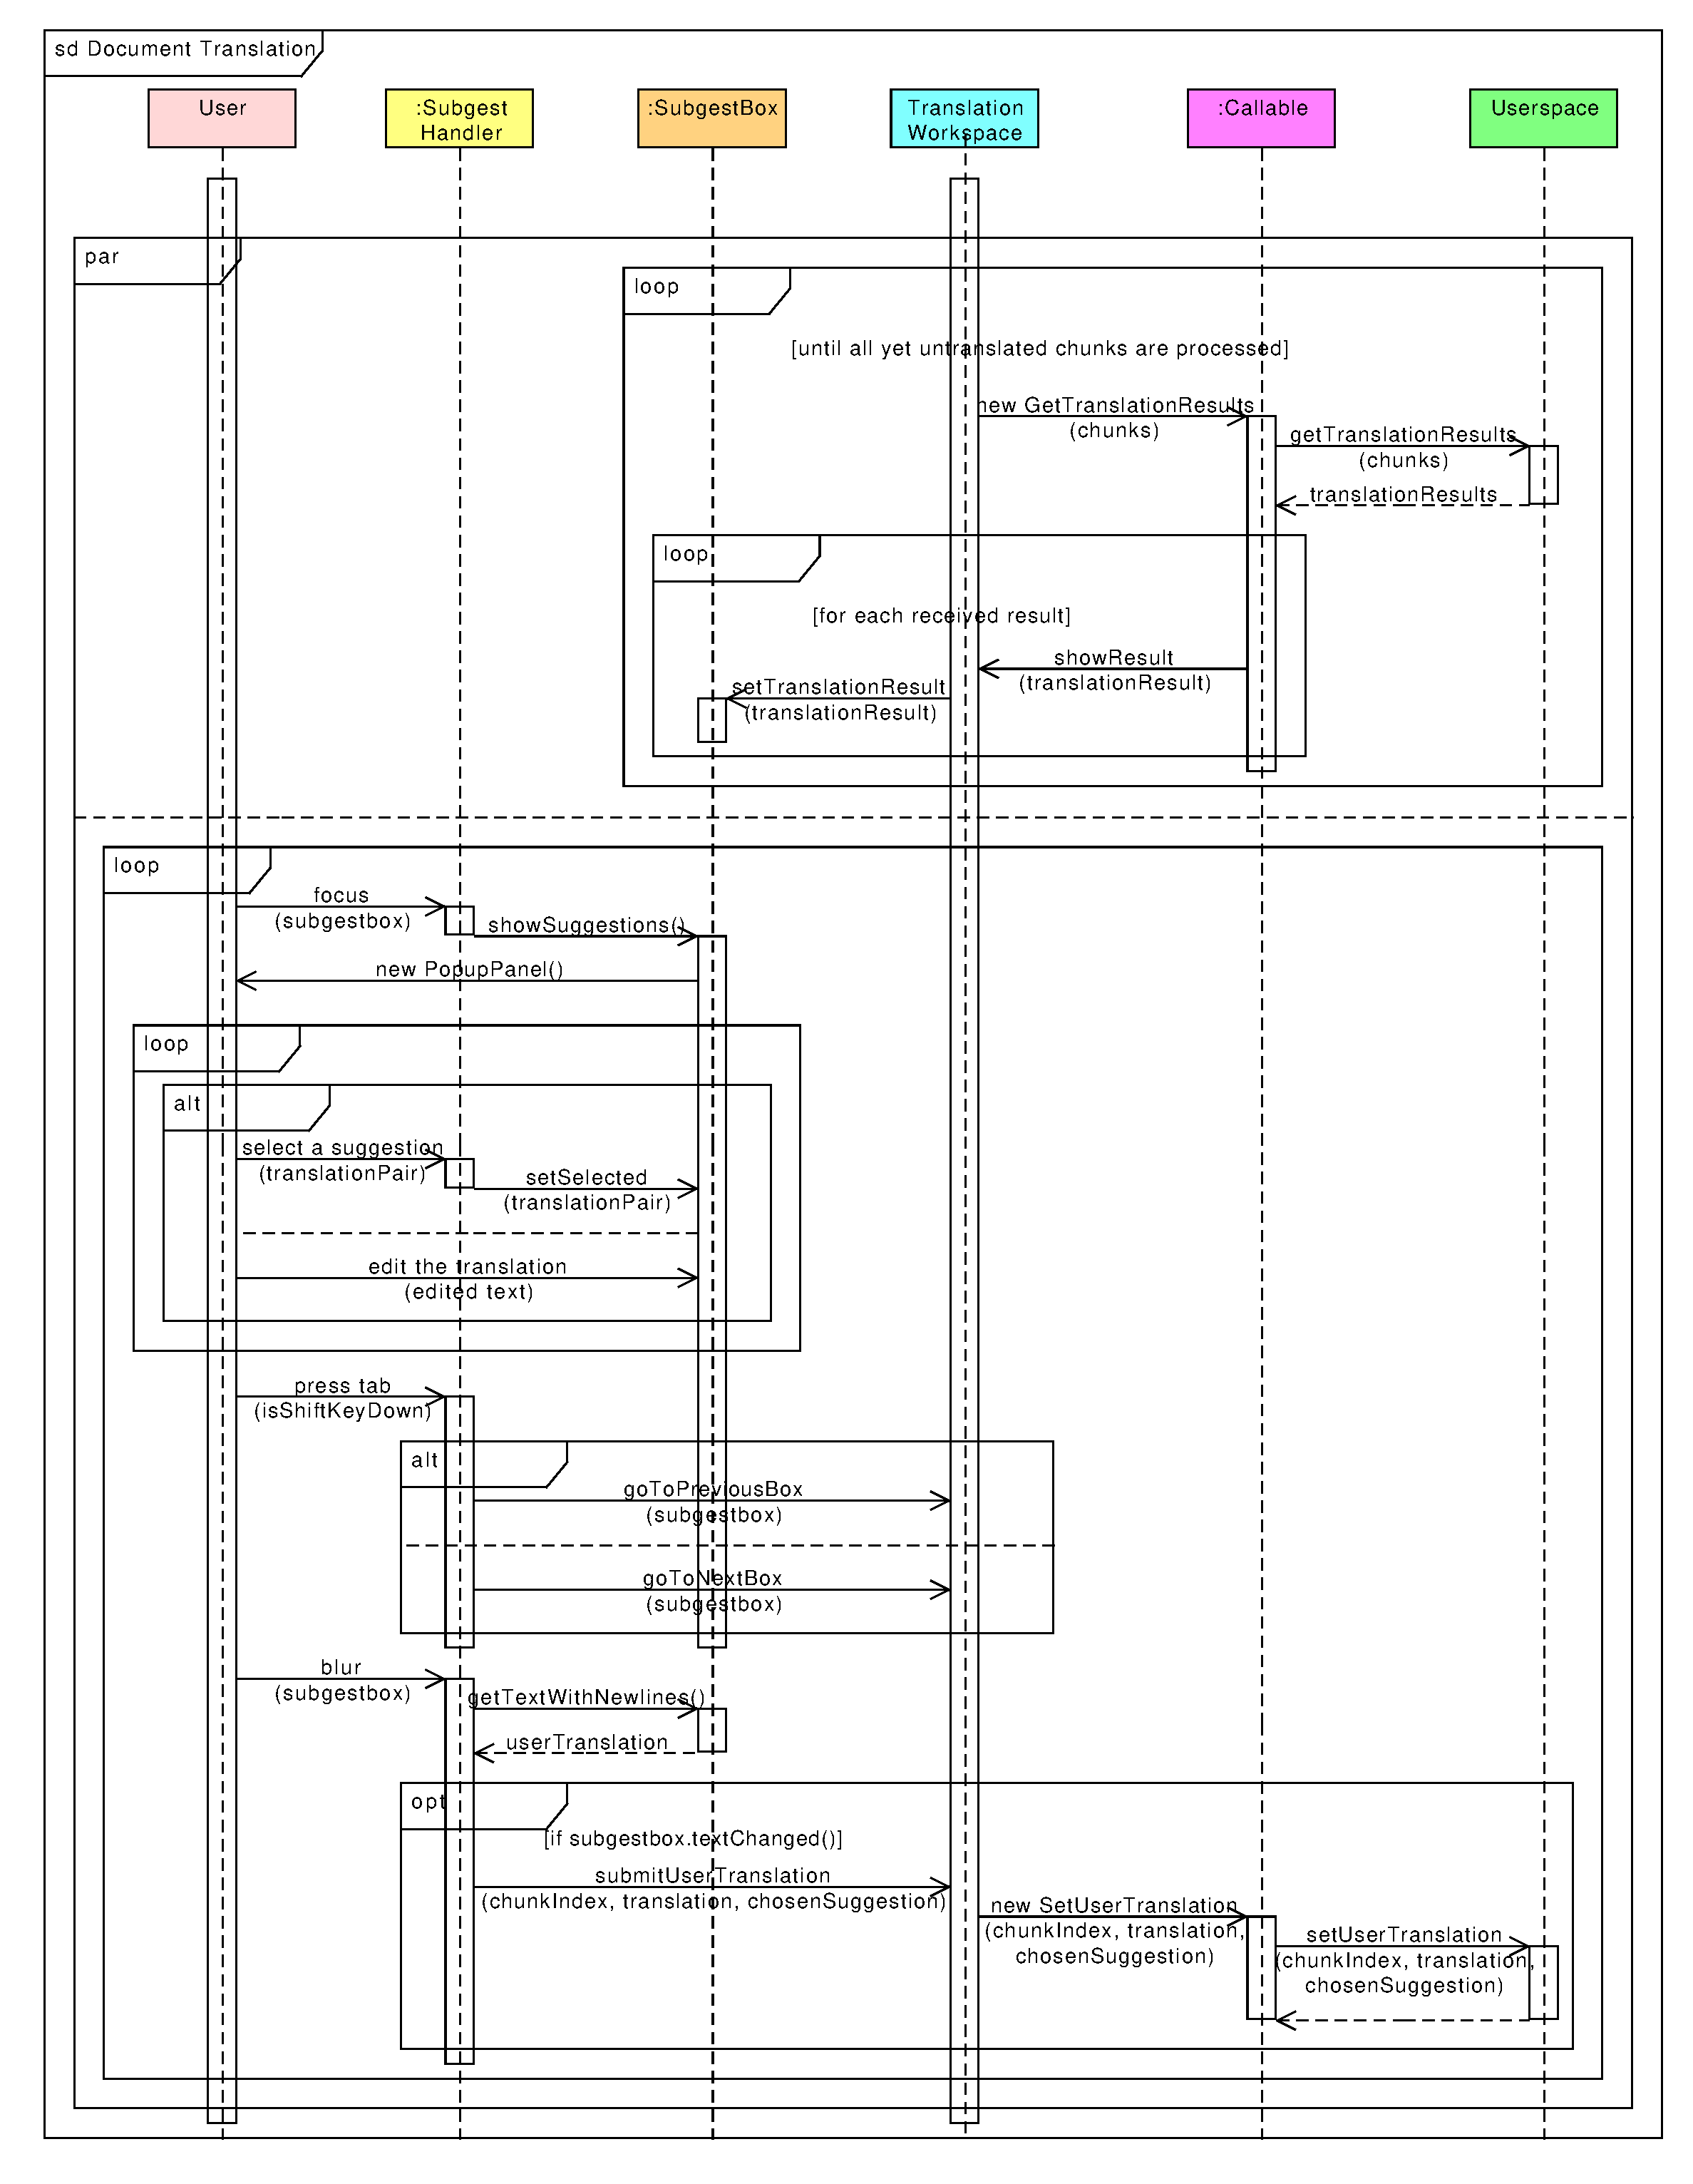
\includegraphics[scale=0.45]{figures/document_translation_sequence.pdf}
\end{center}
\caption{Sequence diagram of document translation.}\label{gui:sd:document_translation}
\end{figure}

\subsection{Document Export}

\todo{I actually dont know how this works.}

\todo{do you want a Sequence Diagram for that? it would be nice but I dont know how we do it, I would have to look into the code (I hope it is at least commented)}

\todo{but probably this is not GUI but userspace mostly}

When finished with this chunk-after-chunk translation, the whole document can be exported as a subtitle file in the SRT format, or as a text file (without the chunk numbers and timing).

A GET request is sent to the servlet.

The servlet takes this and this, checks this and that, loads the chunks using Hibernate, creates the file like this, and returns that as the contents.

\todo{The user translations are probably harvested by Userspace and Core independently of what the user does -- it probably does not fit into the GUI section at all...}
